\documentclass[12pt,reqno]{article}

\usepackage{amsmath, amssymb, amsfonts, amsbsy, amsthm, latexsym, graphicx, mathrsfs}
\usepackage{bbm}
\usepackage{bm}
\usepackage{forest}
\usepackage{caption}
% \usepackage{algorithm}
\usepackage{algorithm2e}
\usepackage{gensymb}
\usepackage{siunitx}
\usepackage{booktabs}
% \usepackage[table]{xcolor} % For coloring rows and columns
\usepackage{tikz}
\usepackage{hyperref}
\usepackage{listings}
\usepackage{xcolor}
\hypersetup{
    colorlinks=true,
    linkcolor=red,
    urlcolor=blue,
    citecolor=green,
}
\RestyleAlgo{ruled}

\usetikzlibrary{arrows, positioning}

% \lstset{
%   basicstyle=\ttfamily,
%   keywordstyle=\color[rgb]{0.13, 0.13, 0.38}, % Keywords in navy blue
%   commentstyle=\color[rgb]{0.5, 0.5, 0.5}, % Comments in gray
%   stringstyle=\color[rgb]{0.63, 0.13, 0.13}, % Strings in dark red
%   backgroundcolor=\color[rgb]{0.95, 0.95, 0.95}, % Light gray background
%   frame=single,
%   breaklines=true,
%   showstringspaces=false,
% }

%New colors defined below
\definecolor{codegreen}{rgb}{0,0.6,0}
\definecolor{codegray}{rgb}{0.5,0.5,0.5}
\definecolor{codepurple}{rgb}{0.58,0,0.82}
\definecolor{backcolour}{rgb}{0.95,0.95,0.92}

%Code listing style named "mystyle"
\lstdefinestyle{mystyle}{
  backgroundcolor=\color{backcolour},   commentstyle=\color{codegreen},
  keywordstyle=\color{magenta},
  numberstyle=\tiny\color{codegray},
  stringstyle=\color{codepurple},
  basicstyle=\ttfamily\footnotesize,
  breakatwhitespace=false,         
  breaklines=true,                 
  captionpos=b,                    
  keepspaces=true,                 
  numbers=left,                    
  numbersep=5pt,                  
  showspaces=false,                
  showstringspaces=false,
  showtabs=false,                  
  tabsize=2
}

%"mystyle" code listing set
\lstset{style=mystyle}

\usepackage[backend=biber,style=alphabetic]{biblatex}
% Add your .bib file
\addbibresource{refs.bib}


\oddsidemargin  0.0in
\evensidemargin 0.0in
\setlength{\topmargin}{.0in}
\setlength{\textheight}{8.75 true in}
\setlength{\textwidth}{6.5 true in}

\theoremstyle{definition}
\newtheorem{theorem}{Theorem} [section]
\newtheorem{definition}[theorem]{Definition}
\newtheorem{remark}[theorem]{Remark}
\newtheorem{example}[theorem]{Example}

\numberwithin{equation}{section}

\title{Sample Engineering Background}
% selected examples
\author{Quill Healey}

\begin{document}
\maketitle
\tableofcontents

\section*{Document Overview}

% Power in approaching problems with an optimization POV
% comment on the part of each problem and knowing when it is appropriate to talk about math
% mention markov chains and MDPs
% problem explanation depends on length of problem solution
% (the first problem description is long...not all are like this)
% feel free to use the table of contents to find and example that catches your eye
% demonstrates what I know; for more technical readers

\section*{Notation}

\newpage

\section{Function Fitting, Statistical Estimation, and Classification}

\subsection{Markov Chain Transition Probability Estimation}

\subsubsection*{Problem Overview and Upshot}

Markov chains are an important, probabilistic tool that can be found across many disciplines,
either used to model some system directly (like in the following example) or as part of a broader solution
approach (\textit{e.g.} Markov Chain Monte Carlo or Markov Decision Processes). We'll forego the mathematics behind Markov chains and consider the canonical weather example.\\
\noindent We suppose on any given day it can be sunny, cloudy, or rainy. This is referred to as the \textit{state}. 
The important assumption we make is that the \textbf{weather tomorrow only depends on the weather today}.
However, given the weather today, we do not know for sure what the weather tomorrow will be, \textit{i.e.} we transition
randomly between states. Figure~\ref{fig:markov} is an example of weather-modeling Markov chain. According to this model,
if it is sunny today, it will be rainy tomorrow with probability 0.1, cloudy tomorrow with probability 0.3,
or sunny again tomorrow with probability 0.6.  

\begin{figure}[htbp]
    \centering
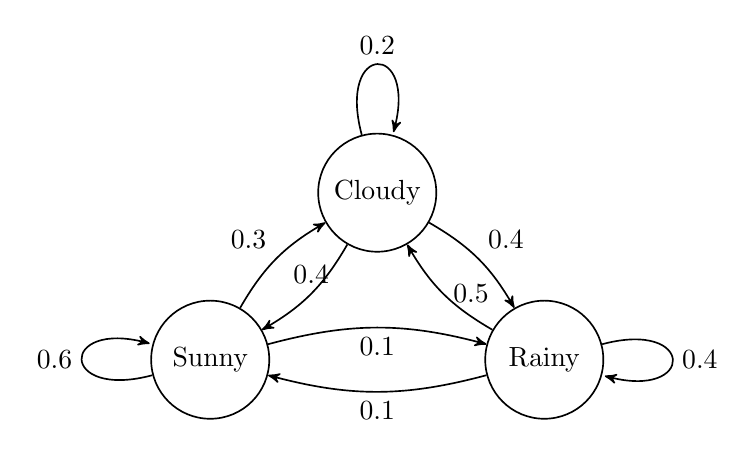
\begin{tikzpicture}[->, >=stealth', auto, semithick, node distance=3cm]
    \tikzstyle{state}=[circle, draw, minimum size=1.5cm, fill=none, text centered]
    
    \node[state]    (S)                     {Sunny};
    \node[state]    (C) [above right of=S]  {Cloudy};
    \node[state]    (R) [below right of=C]  {Rainy};
    
    \path
    (S) edge[bend left=15]     node{0.3} (C)
        edge[loop left]     node{0.6} (S)
        edge[bend left=15]     node[below] {0.1} (R)
    (C) edge[bend left=15]     node[above] {0.4} (S)
        edge[loop above]    node{0.2} (C)
        edge[bend left=15]     node{0.4} (R)
    (R) edge[bend left=15]     node[below] {0.1} (S)
        edge[bend left=15]     node[right] {0.5} (C)
        edge[loop right]    node{0.4} (R);
\end{tikzpicture}
    \caption{Markov chain weather model}
    \label{fig:markov}
\end{figure}

The problem in this section is concerned with \textit{estimating} the transition probabilities between states
having \textit{observed} a sequence of states. In other words, it is a \textbf{statistical question}. Perhaps
we wish to create a new weather app because we believe that our Markov model will do a better job \textit{predicting}
the weather than the default app on our phones (a bold assumption). However, while we know what the states in our system
are, we do not know what the transition probabilities are; \textit{i.e.,} our knowledge of the system is represented by Figure~\ref{fig:markov_unknown}.
We could of course \textit{guess} what each probability is, but the better approach is to \textit{collect data}
and then use this data to guess the probabilities (fun fact: statistics used to be called \textit{inverse probability}). 
\begin{figure}[htbp]
    \centering
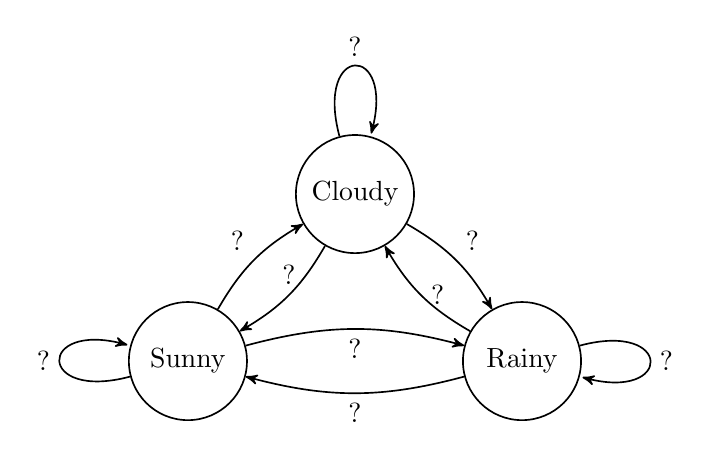
\begin{tikzpicture}[->, >=stealth', auto, semithick, node distance=3cm]
    \tikzstyle{state}=[circle, draw, minimum size=1.5cm, fill=none, text centered]
    
    \node[state]    (S)                     {Sunny};
    \node[state]    (C) [above right of=S]  {Cloudy};
    \node[state]    (R) [below right of=C]  {Rainy};
    
    \path
    (S) edge[bend left=15]     node{?} (C)
        edge[loop left]     node{?} (S)
        edge[bend left=15]     node[below] {?} (R)
    (C) edge[bend left=15]     node[above] {?} (S)
        edge[loop above]    node{?} (C)
        edge[bend left=15]     node{?} (R)
    (R) edge[bend left=15]     node[below] {?} (S)
        edge[bend left=15]     node[right] {?} (C)
        edge[loop right]    node{?} (R);
    
    \end{tikzpicture}
    \caption{Markov chain weather model with unknown transition probabilities}
    \label{fig:markov_unknown}
\end{figure}


For instance, perhaps we kept
track of the weather over the past week and observed that on Monday it rained, on Tuesday it was cloudy,
on Wednesday it was sunny, sunny again on Thursday, cloudy on Friday, and then it rained on both Saturday and
Sunday. The methodology introduced in the problem below would be one way of estimating the probability links
in the above state diagram.

\noindent \textbf{Notes:} 
\begin{itemize}
    \item This problem uses what Gilbert Strang would refer to as a \textit{Markov Matrix}. In 
    more traditional, statistical texts, the transpose of this matrix is worked with, and it is called a \textit{stochastic matrix}.
    \item There are many other methodologies for approaching this inference problem, almost all of which
    are more accurate the majority all of the time. However, this frequentist maximum likelihood approach is often still used as
    part of these other, better methodologies.
\end{itemize}


\subsubsection*{Problem}
~\cite{boyd_convex_optimization} \textbf{Exercise 7.5}. \textit{Markov chain estimation}. Consider a Markov chain
with $n$ states and a trasition probabilty matrix $P \in \mathbf{R}^{n \times n}$ defined as
\[P_{ij} = \mathbf{Prob}\left(y_{t+1} = i \mid y_t = j\right).\]
The transition probabilities must satisfy $P_{i j} \geq 0$ and $\sum_{i=1}^n P_{i j}=1, j=1, \ldots, n$. We consider the problem of estimating the transition probabilities,
given an observed sample sequence $y_1=k_1, y_2=k_2, \ldots, y_N=k_n$.

\vspace{0.1cm}
\noindent (a) Show that if there are no other prior constraints on $P_{i j}$, then the ML estimates are the empirical transition frequencies:
$\hat{P}_{i j}$ is the ratio of the number of times the state transitioned from $j$ into $i$, divided by the number of times it was $j$, in the observed sample.

\vspace{0.1cm}
\noindent (b) Suppose that an equilibrium distribution $p$ of the Markov chain is known, i.e., a vector $q \in \mathbf{R}_{+}^n$ satisfying $\mathbf{1}^T q=1$ and $P q=q$. Show that the problem of computing the ML estimate of $P$,
given the observed sequence and knowledge of $q$, can be expressed as a convex optimization problem.

\subsubsection*{My Response}
\noindent (a) Firstly, we'll let

\[p_{P}(k) = \mathbf{Prob}_{y \sim P}\left(y_1 = k_1, \ldots, y_N = k_n\right)\]
denote either the \textit{joint probability density function} of the observed states, or,
the \textit{likelihood function} of the density parameters given observed states. Which it is depends on context.
Since we are in a statistical setting, it is the likelihood function. Furthermore, we seek to find an estimate
of the transition probabilities between the states of our Markov chain, \textit{i.e.}, we wish to find $\hat{P} \in \mathbf{R}^{n \times n}$.
As specified above, for this problem we will find this estimate using maximum likelihood estimation, corresponding to 

\[\hat{P} = \underset{P}{\mathrm{argmax}} \; p_P(k). \]
We first expand the likelihood function using \textit{the chain rule}

\[ \begin{aligned}
    p_{P}(k) &= \mathbf{Prob}\left(y_{N} = k_n \mid y_{N-1} = k_{n-1}\right) \mathbf{Prob}\left(y_{N-1}=k_{n-1} \mid y_{N-2} = k_{n-2} \right)\\
&\cdots \mathbf{Prob}(y_{2} = k_{2} \mid y_{1} = y_{1}) \mathbf{Prob}\left(y_1 = k_1\right),
\end{aligned} \]
and then use our \textit{Markov} assumption to simplify this expression to

\[p_{P}(k) = P_{k_{n}k_{n-1}}P_{k_{n-1}k_{n-2}} \cdots P_{k_{2}k_{1}},\]
which is simply a product of probabilities, \textit{i.e.}, $P_{ij} \in \mathbf{R}$ (and we assume
that we start in state $k_1$). Letting $c_{ij}$ be the \textit{number of times the state transitioned
from $j$ to $i$}, the likelihoood function becomes
\[p_{P}(k) = \prod_{i, j=1}^{n}P_{ij}^{c_{ij}}.\]
For tractability purposes we now make use of the \textit{log-likelihood function}, which is simply

\[l(P) = \log \left( \prod_{i, j=1}^{n}P_{ij}^{c_{ij}} \right) = \sum_{i, j=1}^{n} c_{ij}\log P_{ij}.\]
To find the transition probability matrix $P$ which maximizes the likelihood of our observed data having occurred,
we thus want to solve
\[\begin{array}{lll}
\text{maximize} \; & \sum_{i, j=1}^{n} c_{ij}\log P_{ij} & \\
\text{subject to} & \bm{1}^T P = 1.
\end{array}\]
(It is critical to formulate this \textit{constrained problem}. Forgetting to include the constraint
is a common mistake which leads to an underdetermined problem.)

\noindent To solve this equality-constrained optimization problem we simply form the Lagrangian

\[L(P, \nu) = \sum_{i, j=1}^{n} c_{ij}\log P_{ij} + \sum_{j=1}^{n} \left(\nu_j \sum_{i=1}^{n}P_{ij} \right),\]
find the partial derivatives of $L$ with respect to some probability ($P_{ij}$)

\[\frac{\partial L}{\partial P_{ij}}(P, \nu) = \frac{c_{ij}}{P_{ij}} + v_{j}\]
and set $\frac{\partial L}{\partial P_{ij}}(P, \nu)$ equal to zero:
\[\frac{c_{ij}}{P_{ij}} = - \nu_j \quad \Longleftrightarrow \quad P_{ij} = \frac{-c_{ij}}{v_{j}}.\]

\noindent Then, plugging this expression for $P_{ij}$ into the constraint 
\[\bm{1}^T P = 1 \Longleftrightarrow \sum_{i=1}^{n}P_{ij}, \quad j = 1, \ldots n,\]
we find that
\[\sum_{i=1}^{n}\frac{-c_{ij}}{v_{j}} = 1, \quad j= 1, \ldots n \quad \Longleftrightarrow \quad v_j = \sum_{i=1}^{n}-c_{ij}, \quad j = 1, \ldots n.\]
Therefore, our final expression for any transition probability is
\[\begin{aligned}
    \hat{P}_{ij} = \frac{-c_{ij}}{v_{j}} = \frac{-c_{ij}}{\sum_{i=1}^{n}-c_{ij}} = \frac{c_{ij}}{\sum_{i=1}^{n}c_{ij}},
\end{aligned}\]
which is of course the empirical transition probability, as desired.

\noindent Note that since this is a convex optimization problem (concave objective function constrained to a convex set)
we don't need to check boundary conditions.
% since this is a convex optimization problem (concave objective function constrained to a convex set) don't need to check boundaries, etc.

\vspace{0.1cm}
\noindent (b) To incorporate additional information about the transition probabilities that we are trying to estimate,
we formulate

\[\begin{array}{lll}
    \text{maximize} \; & \sum_{i, j=1}^{n} c_{ij}\log P_{ij} & \\
    \text{subject to} & \bm{1}^T P = 1 & \\
    & Pq = q,
    \end{array}\]
which is still a convex problem. If we wanted to, we could augment the above Lagrangian with
these additional constraints and find an analytical expression for this problem, but since it is not
required, we can be satisfied knowing that CVXPY could solve this problem with even non-trivial scale data
in under a second.

\subsection{Generative Additive Model}

\subsubsection*{Problem Overview and Upshot}
This problem is straightforward (albeit the model is less so): we wish to \textit{guess} the value
of a function which happens to be some combination of other functions and additional \textit{randomness}.
This is the setup of modern machine learning. There are many other ML models that will
give a better estimate of the underlying function, but a benefit to this model is that
the problem being solved to create it is \textit{convex}, which means that we could embed the corresponding software
onto an online system that observes and reacts to data that the function produces without worrying about
the software failing. 

\subsubsection*{Problem}
~\cite{EE364a-extra}\textbf{Exercise 6.17}. \textit{Fitting a generalized additive regression model}.
A \textit{generalized additive model} has the form
\[
f(x)=\alpha+\sum_{j=1}^n f_j\left(x_j\right)
\]
for $x \in \mathbf{R}^n$, where $\alpha \in \mathbf{R}$ is the offset, and $f_j: \mathbf{R} \rightarrow \mathbf{R}$, with $f_j(0)=0$.
The functions $f_j$ are called the regressor functions. When each $f_j$ is linear, i.e., has the form $w_j x_j$,
the generalized additive model is the same as the standard (linear) regression model.
Roughly speaking, a generalized additive model takes into account nonlinearities in each regressor $x_j$, but not nonlinear interactions among the regressors.
To visualize a generalized additive model, it is common to plot each regressor function (when $n$ is not too large).
We will restrict the functions $f_j$ to be piecewise-affine, with given knot points $p_1<\cdots<p_K$. This means that $f_j$ is affine on the intervals
$\left(-\infty, p_1\right],\left[p_1, p_2\right], \ldots,\left[p_{K-1}, p_K\right],\left[p_K, \infty\right)$, and continuous at $p_1, \ldots, p_K$.
Let $C$ denote the total (absolute value of) change in slope across all regressor functions and all knot points.
The value $C$ is a measure of nonlinearity of the regressor functions; when $C=0$, the generalized additive model reduces to a linear regression model.
Now suppose we observe samples or data $\left(x^{(1)}, y^{(1)}\right), \ldots,\left(x^{(N)}, y^{(N)}\right) \in \mathbf{R}^n \times \mathbf{R}$,
and wish to fit a generalized additive model to the data. We choose the offset and the regressor functions to minimize
\[
\frac{1}{N} \sum_{i=1}^N\left(y^{(i)}-f(x^{(i)})\right)^2+\lambda C.
\]
where $\lambda>0$ is a regularization parameter. (The first term is the mean-square error.)

\vspace{0.1cm}
\noindent (a) Explain how to solve this problem using convex optimization.

\vspace{0.1cm}
\noindent (b) Carry out the method of part (a) using the data in the file \lstinline|gen_add_reg_data.m|. This file contains the data, given as an $N \times n$ matrix $\mathrm{X}$
(whose rows are $\left(x^{(i)}\right)^T$ ), a column vector $\mathrm{y}$ (which give $y^{(i)}$ ), a vector $\mathrm{p}$ that gives the knot points, and the scalar lambda.
Give the mean-square error achieved by your generalized additive regression model.
Compare the estimated and true regressor functions in a $3 \times 3$ array of plots (using the plotting code in the data file as a template), over the range $-10 \leq x_i \leq 10$. The true regressor functions (to be used only for plotting, of course) are given in the cell array $f$.

\subsubsection*{My Response}

\noindent (a) The critical step to using convex optimization to solve this problem is recognizing that
we wish to adjust the value of $\theta \in \mathbf{R}^{n(K+1)}$, where these function parameters 
are found in the feature mappings according to

\[f_{j}(x) = \sum_{k=0}^{K}\theta_{nk + j} b_k(x),\]
where $b_k(x) = \max\{x-p_k, 0\} + \min\{p_k, 0\}$.
Furthermore, letting
\[C = \sum_{j=1}^{n(K+1)} \left| \theta_j \right| = \left\lVert \theta \right\rVert_{1},\]
the following unconstrained optimization problem
\[\mathrm{minimize} \quad \frac{1}{N} \sum_{i=1}^{N}\left(y^{(i)} - (\alpha + \sum_{j=1}^{n}f_j(x_j^{(i)}) ) \right)^2 + \lambda C,\]
is convex.

\noindent (b) The code in algorithm~\ref{alg:gen-add} carries out this method, with the key functionality
functionality coming from the augmented data matrix (numpy matrix \lstinline|Z|). The fit generalized additive
model has a MSE of $0.96962$. A comparision of the estimated and true regressor functions can be found in
figure~\ref{fig:gen_add_fit}.

\begin{algorithm}[htbp]
    \caption{Generalized additive regression model}
    \centering
        \begin{lstlisting}[language=Python]
            Z = X.copy()
            for i in range(K):
                Z = np.hstack((Z, np.maximum(X-p[i], 0) + np.minimum(p[i], 0)))

            theta = cp.Variable(n*(K+1))
            alpha = cp.Variable(1)

            C = cp.norm(theta, 1)
            f0 = 1/N*cp.sum_squares(y - alpha - Z@theta)

            prob = cp.Problem(cp.Minimize(f0 + lambda_value*C), [])
            prob.solve()
        \end{lstlisting}
    \label{alg:gen-add}
\end{algorithm}

\begin{figure}[htbp]
    \centering
    \includegraphics[width=\linewidth]{../examples/364a/cvx-ch7/gen_add_regr_fit.png}
    \caption{True versus Estimated Regressor Functions.}
    \label{fig:gen_add_fit}
\end{figure}

\newpage

\subsection{Bounding Object Position}

\subsubsection*{Problem Overview and Upshot}
The objective of this problem is straightforward: we have some number of cameras observing
a physical space. For illustrative purposes, perhaps these cameras are part of a \textit{targeting system}.
Furthermore, suppose that there's an object in this physical space that we wish to terminate. It is desirable
that we can identify the physical coordinates that this object occupies. The difficulty is that while the object
is in three dimensional space, the image plane is two dimensional. The following
problem dives into the mathematical relationship between image space and physical space to create the tools
necessary to use the images that the cameras take to find the smallest possible box in physical space which this object occupies.

\subsubsection*{Problem}

~\cite{EE364a-extra}\textbf{Exercise 8.8}. \textit{Bounding object position from multiple camera views}.
$x \in \mathbf{R}^3$, and viewed by a set of $m$ cameras. Our goal is to find a box in $\mathbf{R}^3$,
\[
\mathcal{B}=\left\{z \in \mathbf{R}^3 \mid l \preceq z \preceq u\right\},
\]
for which we can guarantee $x \in \mathcal{B}$. We want the smallest possible such bounding box. (Although it doesn't matter, we can use volume to judge 'smallest' among boxes.)

\noindent Now we describe the cameras. The object at location $x \in \mathbf{R}^3$ creates an image on the image plane of camera $i$ at location
\[
v_i=\frac{1}{c_i^T x+d_i}\left(A_i x+b_i\right) \in \mathbf{R}^2 .
\]

\noindent The matrices $A_i \in \mathbf{R}^{2 \times 3}$, vectors $b_i \in \mathbf{R}^2$ and $c_i \in \mathbf{R}^3$, and real numbers $d_i \in \mathbf{R}$ are known, and depend on the camera positions and orientations. We assume that $c_i^T x+d_i>0$. The $3 \times 4$ matrix
\[
P_i=\left[\begin{array}{ll}
A_i & b_i \\
c_i^T & d_i
\end{array}\right]
\]
is called the camera matrix (for camera $i$ ). It is often (but not always) the case the that the first 3 columns of $P_i$ (i.e., $A_i$ stacked above $c_i^T$ ) form an orthogonal matrix, in which case the camera is called orthographic.
We do not have direct access to the image point $v_i$; we only know the (square) pixel that it lies in. In other words, the camera gives us a measurement $\hat{v}_i$ (the center of the pixel that the image point lies in); we are guaranteed that
\[
\left\|v_i-\hat{v}_i\right\|_{\infty} \leq \rho_i / 2,
\]
where $\rho_i$ is the pixel width (and height) of camera $i$. (We know nothing else about $v_i$; it could be any point in this pixel.)
Given the data $A_i, b_i, c_i, d_i, \hat{v}_i, \rho_i$, we are to find the smallest box $\mathcal{B}$ (i.e., find the vectors $l$ and $u$ ) that is guaranteed to contain $x$.
In other words, find the smallest box in $\mathbf{R}^3$ that contains all points consistent with the observations from the camera.

\vspace{0.1cm}
\noindent (a) Explain how to solve this using convex or quasiconvex optimization. You must explain any transformations you use, any new variables you introduce, etc.
If the convexity or quasiconvexity of any function in your formulation isn't obvious, be sure justify it.

\vspace{0.1cm}
\noindent (b) Solve the specific problem instance given in the file \lstinline|camera_data.m|. Be sure that your final numerical answer (i.e., $l$ and $u$ ) stands out.

\subsubsection*{My Response}

$x$ is some object in the physical world (modeled as 3-dimensional Euclidean space). We have $m$ cameras which capture images
of $x$. However, because

Let's first formulate the constraints ensuring that our proposed box that $x$ lies in is consistent with the camera measurements;
\textit{i.e.}, there isn't a point in the bounding box which contra

\[\left\lVert v_i - \hat{v}_i \right\rVert_{\infty} \le \rho_i / 2, , \quad i = 1, \ldots, m\]
is expanded as 
\[\left\lVert \frac{1}{c_i^T x+d_i}\left(A_i x+b_i\right) - \hat{v}_i \right\rVert_{\infty} \le \rho_i/2, \quad i = 1, \ldots, m.\]
The $\ell_{\infty}$-norm is requiring that the absolute value of both terms in the $\mathbf{R}^2$ vector
\[\frac{1}{c_i^T x+d_i}\left(A_i x+b_i\right) - \hat{v}_i\]
be less than or qual to $\rho_i/2$. Furthermore,

\[-(\rho_i/2) \bm{1} \preceq \frac{1}{c_i^T x+d_i}\left(A_i x+b_i\right) - \hat{v}_i \preceq (\rho_i/2) \bm{1}, \quad i = 1, \ldots, m\]

\[(\hat{v}_i - (\rho_i/2) \bm{1})(c_i^T x + d_i) \preceq A_i x + b_i \preceq (\hat{v}_i + (\rho_i/2))(c_i^Tx + d_i), \quad i = 1, \ldots, m\]

\subsection{Robust Logistic Regression}

\subsubsection*{Problem Overview and Upshot}
The logistic regression framework is a typical classification problem approach. As an example,
perhaps a drone is collecting terrain data 

\subsubsection*{Problem}

~\cite{EE364a-extra} \textbf{Exercise 6.29}. \textit{Robust Logistic Regresion}.
We are given a dataset $x_i \in \mathbf{R}^d$, $y_i \in \left\{ -1, 1 \right\}$, $i = 1, \ldots, n$.
We seek a prediction model $y \approx \hat{y}=\operatorname{sign}\left(\theta^1 x\right)$, where $\theta \in \mathbf{R}^a$ is the model parameter. In logistic regression, $\theta$ is chosen as the minimizer of the logistic loss
\[
\ell(\theta)=\sum_{i=1}^n \log \left(1+\exp \left(-y_i \theta^T x_i\right)\right)
\]
which is a convex function of $\theta$. (We will assume that a minimizer exists.)

\noindent We will take into account the idea that the feature vectors $x_i$ are not known precisely.
Specifically we imagine that each entry of each feature vector can vary by $\pm \epsilon$, where $\epsilon>0$ is a given uncertainty level.
We define the worst-case logistic loss as
\[
\ell^{\mathrm{wc}}(\theta)=\sum_{i=1}^n \sup _{\left\|\delta_i\right\|_{\infty} \leq \epsilon} \log \left(1+\exp \left(-y_i \theta^T\left(x_i+\delta_i\right)\right)\right) .
\]

\noindent In words: we perturb each feature vector's entries by up to $\epsilon$ in such a way as to make the logistic loss as large as possible. Each term is convex, since it is the supremum of a family of convex functions of $\theta$, and so $\ell^{\mathrm{wc}}(\theta)$ is a convex function of $\theta$.

\vspace{0.1cm}
\noindent In \textit{robust logistic regression}, we choose $\theta$ to minimize $\ell^{\mathrm{wc}}(\theta)$.
(Here too we assume a minimizer exists.)

\vspace{0.1cm}
\noindent (a) Explain how to carry out robust logistic regression by solving a single convex optimization problem in disciplined convex programming (DCP) form.
Justify any change of variables or introduction of new variables.
Explain why solving the problem you propose also solves the robust logistic regression problem.\\
\noindent Hint: $\log (1+\exp (u))$ is monotonic in $u$.

\vspace{0.1cm}
\noindent (b) Fit a logistic regression model (i.e., minimize $\ell(\theta)$ ), and also a robust logistic regression model
(i.e., minimize $\ell^{\mathrm{wc}}(\theta)$ ), using the data given in \lstinline|rob_logistic_reg_data.py|.
The $x_i \mathrm{~s}$ are provided as the rows of a $n \times d$ matrix named $\mathrm{x}$.
The $y_i \mathrm{~s}$ are provided as the entries of a $n$ vector named $\mathrm{y}$.
The file also contains a test data set, \lstinline|x_test|, \lstinline|y_test|. Give the test error rate (i.e., fraction of test set data points for which $\hat{y} \neq y$ )
for the logistic regression and robust logistic regression models.

\subsubsection*{My Response}

\noindent We will consider a generalization of this problem. Specifically, we'll actually define the worst-case logistic loss as

\[
\ell^{\mathrm{wc}}(\theta)=\sum_{i=1}^n \sup _{\left\|\delta_i\right\| \leq \epsilon} \log \left(1+\exp \left(-y_i \theta^T\left(x_i+\delta_i\right)\right)\right),
\]
where $\left\lVert \delta_i \right\rVert$ is just \textit{some norm} on $\mathbf{R}^{d}$. We will explore the reasoning behind
this generalization after reformulating the model.

\noindent The robust logistic regression problem is to solve the unconstrained problem

\[\mathrm{minimize} \quad \ell^{\mathrm{wc}}(\theta)=\sum_{i=1}^n \sup _{\left\|\delta_i\right\| \leq \epsilon} \log \left(1+\exp \left(-y_i \theta^T\left(x_i+\delta_i\right)\right)\right);\]
however, while this \textit{is} a convex optimization problem, \textit{it is not} DCP compatible. This is because
the supremum operator is an analytical expression; \textit{i.e.,} (for our purposes), it cannot be handled by a computer.
Furthermore, we need to reformulate the problem so the supremum operator is neither in the objective function nor in any
constraint function. To begin reformulating, we use the hint and move the supremum from the objective function
to the constraint set. The corresponding problem is,

\[\begin{array}{lll}
\text{minimize} \; & \sum_{i=1}^n \log \left(1+\exp \left(u_i\right)\right) & \\
\text{subject to} & \sup \left\{-y_i \theta^T\left(x_i+\delta_i\right) \mid \left\lVert \delta_i \right\rVert \le \epsilon \right\} \le u_i, \; & i = 1, \ldots, n,
\end{array}\]
where now both $\theta \in \mathbf{R}^d$ and $u \in \mathbf{R}^n$ are optimization variables.
To see that this problem is equivalent to the original unconstrained problem, consider holding $\theta$ fixed
and optimizing solely over $u$. Because the log-sum-exp function is monotonic in its input and the objective function
is separable, we achieve the optimum over $u$ by choosing
\[u_i = \sup \left\{-y_i \theta^T\left(x_i+\delta_i\right) \mid \left\lVert \delta_i \right\rVert \le \epsilon \right\} \]
for $i = 1, \ldots n$. Furthermore, then optimizing over $\theta$ yields the original, unconstrained problem.

Now, as previously mentioned, having the supremum operator in the constraint function set does not
make the problem DCP compatible. Furthermore, we continue and finish the reformulation effort by first
pulling terms out of the supremum:
\[\sup \left\{-y_i \theta^T\left(x_i+\delta_i\right) \mid \left\lVert \delta_i \right\rVert \le \epsilon \right\} \le u_i, \quad i = 1, \ldots, n,\]
is equivalent to
\[-y_i\theta^Tx_i + \sup \left\{ -y_i \theta^T \delta_i \mid \left\lVert \delta_i \right\rVert \le \epsilon \right\} \le u_i \quad i = 1, \ldots, n,\]
and then scaling the expression within the supremum
to recognize that 
\[\sup \left\{ -y_i \theta^T \delta_i \mid \left\lVert \delta_i \right\rVert \le \epsilon \right\} = \sup \left\{ -\epsilon y_i \theta^T \delta_i \mid \left\lVert \delta_i \right\rVert \le 1 \right\} = \left\lVert -\epsilon y_i \theta \right\rVert_{*},\]
where $\left\lVert \cdot \right\rVert_{*}$ is the \textit{dual norm} of whatever norm we choose to define our uncertainty set.
Therefore, we've found that our original unconstrained, non-DCP compatible robust logistic regression optimization problem
\[\mathrm{minimize} \quad \ell^{\mathrm{wc}}(\theta)=\sum_{i=1}^n \sup _{\left\|\delta_i\right\| \leq \epsilon} \log \left(1+\exp \left(-y_i \theta^T\left(x_i+\delta_i\right)\right)\right)\]
is equivalent to the following constrained, DCP compatible robust logistic regression optimization problem
\[\begin{array}{lll}
    \text{minimize} \; & \sum_{i=1}^n \log \left(1+\exp \left(u_i\right)\right) & \\
    \text{subject to} & -y_i\theta^Tx_i + \left\lVert -\epsilon y_i \theta \right\rVert_{*} \le u_i, \; & i = 1, \ldots, n.
    \end{array}\]

\noindent It turns out that the choice of uncertainty set (induced by our choice in norm) dramatically affects the accuracy of this robust model.
In table~\ref{tab:logistic-percent} one can find the test error rate of a typical logistic regression model versus
robust logistic regression models with uncertainty sets induced by $\ell_1$-, $\ell_2$-, and $\ell_\infty$-norms
and varying values of $\theta$. In most every circumstance, at least one, if not all, of the robust models perform
better than the vanially model (and sometimes significantly so). Table~\ref{tab:logistic} contains the raw
classification scores of each model for each $\epsilon$ for a test data set containing $n=60$ points.
% Conceptually,
% choosing a 
% \begin{itemize}
%     \item $\ell_2$-norm corresponds to saying that a data point $x_i \in \mathbf{R}^d$ 
%     can lie in a Euclidean ball uncertainty set with radius $\epsilon$,
%     \item $\ell_1$-norm corresponds to saying that a data point $x_i \in \mathbf{R}^d$ 
%     can lie in a box uncertainty set with radius $\epsilon$,
% \end{itemize} 


    \begin{table}[h]
        \centering
        \begin{tabular}{|c|c|c|c|}
            \hline
            & $\epsilon = 0.5$ & $\epsilon = 0.75$ & $\epsilon = 1$ \\
            \hline
            Non-Robust & \multicolumn{1}{>{\centering\arraybackslash}m{3cm}|}{36} & \multicolumn{1}{>{\centering\arraybackslash}m{3cm}|}{39} & \multicolumn{1}{>{\centering\arraybackslash}m{3cm}|}{35} \\
            \hline
            $\ell_1$ Uncertainty & \multicolumn{1}{>{\centering\arraybackslash}m{3cm}|}{47} & \multicolumn{1}{>{\centering\arraybackslash}m{3cm}|}{44} & \multicolumn{1}{>{\centering\arraybackslash}m{3cm}|}{35} \\
            \hline
            $\ell_2$ Uncertainty & \multicolumn{1}{>{\centering\arraybackslash}m{3cm}|}{49} & \multicolumn{1}{>{\centering\arraybackslash}m{3cm}|}{47} & \multicolumn{1}{>{\centering\arraybackslash}m{3cm}|}{41} \\
            \hline
            $\ell_\infty$ Uncertainty & \multicolumn{1}{>{\centering\arraybackslash}m{3cm}|}{37} & \multicolumn{1}{>{\centering\arraybackslash}m{3cm}|}{46} & \multicolumn{1}{>{\centering\arraybackslash}m{3cm}|}{41} \\
            \hline
        \end{tabular}
        \caption{Number of Correct Classifications out of $n=60$}
        \label{tab:logistic}
    \end{table}

    \begin{table}[h]
        \centering
        \begin{tabular}{|c|c|c|c|}
            \hline
            & $\epsilon = 0.5$ & $\epsilon = 0.75$ & $\epsilon = 1$ \\
            \hline
            Non-Robust & \multicolumn{1}{>{\centering\arraybackslash}m{3cm}|}{0.6} & \multicolumn{1}{>{\centering\arraybackslash}m{3cm}|}{0.65} & \multicolumn{1}{>{\centering\arraybackslash}m{3cm}|}{0.583} \\
            \hline
            $\ell_1$ Uncertainty & \multicolumn{1}{>{\centering\arraybackslash}m{3cm}|}{0.783} & \multicolumn{1}{>{\centering\arraybackslash}m{3cm}|}{0.733} & \multicolumn{1}{>{\centering\arraybackslash}m{3cm}|}{0.583} \\
            \hline
            $\ell_2$ Uncertainty & \multicolumn{1}{>{\centering\arraybackslash}m{3cm}|}{0.817} & \multicolumn{1}{>{\centering\arraybackslash}m{3cm}|}{0.783} & \multicolumn{1}{>{\centering\arraybackslash}m{3cm}|}{0.683} \\
            \hline
            $\ell_\infty$ Uncertainty & \multicolumn{1}{>{\centering\arraybackslash}m{3cm}|}{0.617} & \multicolumn{1}{>{\centering\arraybackslash}m{3cm}|}{0.767} & \multicolumn{1}{>{\centering\arraybackslash}m{3cm}|}{0.683} \\
            \hline
        \end{tabular}
        \caption{Test Error Rate}
        \label{tab:logistic-percent}
    \end{table}

\newpage

\section{Design and Control}

\subsection{Minimum Fuel Control}

\subsubsection*{Problem Overview and Upshot}
While there's some math and optimization techniques involved, the big picture of this problem is very intuitive.
An exampel 
\subsubsection*{Problem}

\noindent~\cite{boyd_convex_optimization} \textbf{Exercise 4.16}. \textit{Minimum fuel optimal control}.
    Consider the LTI dynamical system with state $x_t \in \mathbf{R}^n$, $t = 0, \ldots, N$, and actuator
    or input signal $u_t \in \mathbf{R}$, for $t = 0, \ldots, N-1$. The dynamics of the system are governed by the
    linear recurrence
    \[x_{t+1} = Ax_t + bu_t, \quad t=0, \ldots N-1,\]
    where $A \in \mathbf{R}^{m \times n}$ and $b \in \mathbf{R}^n$ are given. Assume the initial state is $x_0 = 0$.
    The \textit{minimum fuel optimal control problem} is to choose the inputs $u_0, \ldots u_{N-1}$ so as to
    minimize the total fuel consumed, which is given by
    \[F = \sum_{t=0}^{N-1}f(u_t),\]
    subject to the constraint that $x_N = x_{\text{des}}$, where $N$ is the (given) time horizon and
    $x_{\text{des}} \in \mathbf{R}^n$ is the (given) desired final or target state. The function $f: \mathbf{R} \to \mathbf{R}$
    is the \textit{fuel use map} for the actuator, and gives the amount of fuel used as a function of the actuator signal amplitude.
    In this problem we use
    \[f(a) = \begin{cases}
        \left| a \right| & \left| a \right| \le 1 \\
        2 \left| a \right| - 1 & \left| a \right| > 1.
        \end{cases}\]
    Formulate the minimum fuel control problem as an LP. 

\subsubsection*{Response}
    We want to write this minimum
    fuel optimal control problem as a LP. However, a LP formulation is rather restrictive,
    so let's begin by formulating this problem as a convex optimization problem. It is tempting
    to naively claim that the problem
   \[\begin{array}{lll}
   \text{minimize} \; & \sum_{t=0}^{N-1} f(u_t) & \\
   \text{subject to} & x_{t+1} = Ax_t + bu_t, \; & t=0, \ldots, N-1 \\
   & x_0 = 0, \quad x_{N} = x_{\text{des}}.
   \end{array}\]
   is convex. However, we must remember that $f$ is a piecewise function that we are unfamiliar with (\textit{e.g.}
   it isn't a piecwise linear function). Furthermore, this proprosed formulation is not a conex optimization
   problem. Consider the graph of the fuel use map in figure~\ref{fig:fuel-map}. As stated in the legend of this figure,
   and clearly seen when observing the graph,
   the piecewise function $f$ is equivalent to $\max\{\left| a \right|, 2 \left| a \right| - 1\}$.
   (Of course one could also provide an algebraic argument if so desired.) Furthermore, 
   the optimal fuel control problem can be formulated as

   % Important/Helpful to map this back to 4.11
   % Actually, how would you map this to ||Ax-b||_1 approximation
   \begin{figure}[h]
       \centering
       \includegraphics[width=\linewidth]{../examples/364a/cvx-ch4/actuator_fuel-use.pdf}
       \caption{Actuator Fuel Use Map.}
       \label{fig:fuel-map}
   \end{figure}

   \[\begin{array}{lll}
       \text{minimize} \; & \sum_{t=0}^{N-1} \max \left\{ \left| u_t \right|, 2 \left| u_t \right| - 1 \right\} & \\
       \text{subject to} & x_{t+1} = Ax_t + bu_t, \; & t=0, \ldots, N-1 \\
       & x_0 = 0, \quad x_{N} = x_{\text{des}},
       \end{array}\]
   which is a valid convex optimization problem. If our goal was
   simply to find the optimal solution to this fuel problem and we didn't care about 
   formulating the problem as a LP, \textbf{we could end our reformulating here.} In fact,
   the optimal solution $u^* \in \mathbf{R}^{Nm}$, where $Nm = N1 = N$, plotted in figure~\ref{fig:4-16_min-fuel}
   was obtained by solving this convex problem. 
   Nonetheless, we trudge forward with our LP formulation.\\
   For the time being, to be more concise, let's drop the linear dynamical system constraints
   \[x_0 = 0, \; x_N = x_{\text{des}}, \; \text{ and } \; x_{t+1} = Ax_t + bu_t, \quad t = 0, \ldots N-1\]
   and just consider the unconstrained problem
   \[\text{minimize} \; \sum_{t=0}^{N-1} \max \left\{ \left| u_t \right|, 2 \left| u_t \right| - 1 \right\}.\]

   Our first reformulation uses that an objective function defined as the sum of absolute value/maximum expressions can be rewritten
   as a sum of auxilary variables, $s \in \mathbf{R}^N$ here, with each summand being less than
   or equal to an element in the auxilary variable vector. To simplify the problem further we can also 
   remove the max operator from each summand using that if the maximum element in the set
   being operated on by $\max$ is less than or equal to $s_t$, then so must every other element.
   These two reformulation techniques yield the problem

   \[\begin{array}{lll}
   \text{minimize} \; & \bm{1}^T s & \\
   \text{subject to} & \left| u_t \right| \le s_t, & t = 1, \ldots N \\
   & 2 \left| u_t \right| - 1 \le s_t, & t = 1, \ldots N.
   \end{array}\]
   To fully linearize the problem, consider $y \in \mathbf{R}^N$ and the problem

   \[\begin{array}{lll}
   \text{minimize} \; & \bm{1}^T s & \\
   \text{subject to} & y \preceq s & \\
   & 2y - \bm{1} \preceq s \\
   & -y \preceq u \preceq y, & 
   \end{array}\]
   which uses this new variable to ``pull out'' the absolute value from the two other sets
   of constraints.
   Now, before returning the LDS constraints to the formulation observe the pattern in the LDS defining recurrence,

   \[\begin{aligned}
    x_1 &= Ax_0 + bu_0 \\
    x_2 &= Ax_1 + bu_1 \\
    &= A(Ax_0 + bu_0)+ bu_1 = A^2x_0 + Abu_0 + bu_1 \\
    x_3 &= A^3x_0 + A^2b_0 + Abu_1 + bu_2. \\
    &\vdots
    \end{aligned}\]

    Plugging $x_0$ and $x_{\mathrm{des}}$ into the recurrence, the system evolution constraints
    are introduced back into the optimization problem
    
    \[\begin{array}{lll}
        \text{minimize} \; & \bm{1}^T s & \\
        \text{subject to} & Hu = x_{\mathrm{des}} \; &\\
        & y \preceq s & \\
        & 2y - \bm{1} \preceq s & \\
        & -y \preceq u \preceq y, & 
        \end{array}\]

    with the equality constraints $Hu = x_{\mathrm{des}}$, where
    \[H = \begin{bmatrix}
        A^{N-1}b & A^{N-2}b & \cdots & Ab & b
    \end{bmatrix}.\]
    This LP is equivalent to the original minimum fuel optimal control problem, with the corresponding optimal actuator signal
    plotted in figure~\ref{fig:4-16_min-fuel}.
   

   \begin{figure}[htbp]
    \centering
    \includegraphics[width=\linewidth]{../examples/364a/cvx-ch4/4-16_min-fuel.pdf}
    \caption{Minimum fuel actuator signal.}
    \label{fig:4-16_min-fuel}
    \end{figure}

\newpage
\subsection{Path Planning with Contingencies}

\subsubsection*{Problem Overview and Upshot}

The problem is to develop three routes for a vehicle. Two routes are ``contingency routes''
as they address the situation that there's an obstacle in the way of the vehicle which is only
revealed while the vehicle is in motion.

\subsubsection*{Problem}
~\cite{EE364a-extra} \textbf{Exercise 16.9}. \textit{Path Planning with contingencies}.
A vehicle path down a (straight, for simplicity) road is specified
by a vector $p \in \mathbf{R}^N$, where $p_i$ gives the position perpendicular to the centerline at the point $i h$ meters down the road, where $h>0$ is a given discretization size. (Throughout this problem, indexes on $N$-vectors will correspond to positions on the road.)
We normalize $p$ so $-1 \leq p_i \leq 1$ gives the road boundaries. (We are modeling the vehicle as a point, by adjusting for its width.)
You are
given the initial two positions $p_1=a$ and $p_2=b$ (which give the initial road position and angle), as well as the final two positions $p_{N-1}=c$ and $p_N=d$.
You know there may be an obstruction at position $i=O$. This will require the path to either go around the obstruction on the left, which requires $p_O \geq 0.5$,
or on the right, which requires $p_O \leq-0.5$, or possibly the obstruction will clear, and the obstruction does not place any additional constraint on the path.
These are the three contingencies in the problem title, which we label as $k=1,2,3$.
You will plan three paths for these contingencies, $p^{(i)} \in \mathbf{R}^N$ for $i=1,2,3$.
They must each satisfy the given initial and final two road positions and the constraint of staying within the road boundaries.
Paths $p^{(1)}$ and $p^{(2)}$ must satisfy the (different) obstacle avoidance constraints given above. Path $p^{(3)}$ does not need to satisfy an avoidance constraint.
Now we add a twist: You will not learn which of the three contingencies will occur until the vehicle arrives at position $i=S$, when the sensors will determine which contingency holds.
We model this with the information constraints (also called causality constraints or non-anticipatory constraints),
\[
p_i^{(1)}=p_i^{(2)}=p_i^{(3)}, \quad i=1, \ldots, S,
\]
which state that before you know which contingency holds, the three paths must be the same.
The objective to be minimized is
\[
\sum_{k=1}^3 \sum_{i=2}^{N-1}\left(p_{i-1}^{(k)}-2 p_i^{(k)}+p_{i+1}^{(k)}\right)^2,
\]
the sum of the squares of the second differences, which gives smooth paths.

\vspace{0.1cm}
\noindent (a) Explain how to solve this problem using convex optimization.

\vspace{0.1cm}
\noindent (b) Solve the problem with data given in \lstinline|path_plan_contingencies_data.*|. The data files include code to plot the results,
which you should use to plot (on one plot) the optimal paths.
Report the optimal objective value. Give a very brief informal explanation for what you see happening for $i=1, \ldots, S$.
Hint. In Python, use the (default) solver ECOS to avoid warnings about inaccurate solutions.

\subsubsection*{My Response}

Fortunately, the problem as stated is already a DCP compatible optimization problem. The corresponding formulation is

\[\begin{array}{lll}
\text{minimize} \; & \sum_{k=1}^3 \sum_{i=2}^{N-1}\left(p_{i-1}^{(k)}-2 p_i^{(k)}+p_{i+1}^{(k)}\right)^2 & \\
\text{subject to} & p_{i}^{(1)} = p_{i}^{(2)} = p_{i}^{(3)}, & i = 1, \ldots, S \\
& p_{O}^{(1)} \ge 1/2, & \\
& p_{O}^{(2)} \le -1/2, & \\
& p^{(i)}_{1} = a, \quad p^{(i)}_{2} = b, & i = 1, 2, 3 \\
& p^{(i)}_{N-1} = c, \quad p^{(i)}_{N} = d, & i = 1, 2, 3.
\end{array}\]

\noindent (b) The code in algorithm~\ref{alg:path-plan} is all that is required to solve the problem,
\begin{algorithm}[htbp]
    \caption{Path Planning Code}
    \centering
        \begin{lstlisting}[language=Python]
            p = cp.Variable((3, N))

            constrs = [constr for constr_tuple in
                       [(p[0, i] == p[1, i], p[2, i] == p[1, i]) for i in range(2, S+1)]
                       for constr in constr_tuple]
            constrs += [p[0, O] >= h,
                        p[1, O] <= -h]
            constrs += [p[:, 0] == p1*np.ones(3),
                        p[:, 1] == p2*np.ones(3),
                        p[:, N-2] == pN_1*np.ones(3),
                        p[:, N-1] == pN*np.ones(3)]
            
            f0 = cp.sum( [ cp.sum_squares( cp.vstack([p[k, i-1] - 2*p[k, i] + p[k, i+1] for i in range(2, N-2)]) ) for k in range(3)] )
            
            prob = cp.Problem(cp.Minimize(f0), constrs)
            prob.solve()
        \end{lstlisting}
    \label{alg:path-plan}
\end{algorithm}
and when instatiating the model with the provided values, we find $p^* = 0.0001423$ (examining
the paths, this low objective value makes sense as there are no sharp deviations
along any of the paths). 
The optimal paths can be found in figure~\ref{fig:path_plan}. For steps $i=1, \ldots, 60$ we see that
indeed all paths follow the same trajectory, but once the object is revealed, the two contingency paths
make the necessary adjustments to avoid the object.


\begin{figure}[htbp]
    \centering
    \includegraphics[width=\linewidth]{../examples/364a/path_plan_cont.pdf}
    \caption{Possible Paths.}
    \label{fig:path_plan}
\end{figure}

\subsection{Output Tracking}

\subsubsection*{Problem Overview}
This is another problem which is best understood through an example. Specifically,
imagine that we wish 

\subsubsection*{Problem}

\noindent~\cite{EE364b} \textbf{HW7 Q1.}\textit{MPC for output tracking}.  Consider the linear dynamical system
    \[x_{t+1} = Ax_t + Bu_t, \quad y_t = Cx_t, \quad t = 0, \ldots, T-1,\]
    with state $x_t \in \mathbf{R}^n$, input $u_t \in \mathbf{R}^m$, and output $y_t \in \mathbf{R}^p$.
    The matrices $A$ and $B$ are known, and $x_0=0$. The goal is to choose the input sequence $u_1, \ldots, u_t$
    to minimize the output tracking cost
    \[J_{\text{output}} = \sum_{t=1}^{T}\left\lVert y_t - y_t^{\text{des}} \right\rVert_{2}^2,\]
    subject to $\left\lVert u_t \right\rVert_{\infty} \le U^{\text{max}}, \, t=0, \ldots, T-1$. \\
    For the remainder of this problem we work with the specific problem instance with associated data
    \[A = \begin{bmatrix}
        1 & 1 & 0 \\ 0 & 1 & 1 \\ 0 & 0 & 1
    \end{bmatrix}, \quad
    B = \begin{bmatrix}
        0 \\ 0.5 \\ 1
    \end{bmatrix}, \quad
    C = \begin{bmatrix}
        -1 & 0 & 1
    \end{bmatrix},\]
    $T=100$, and $U^{\text{max}} = 0.1$. The desired output trajectory is given by

    \[y^{\text{des}}_t = \begin{cases}
        0 & t < 30, \\
        10 & 30 \le t < 70 \\
        0 & t \ge 70.
    \end{cases}\]

    \noindent (a) Find the optimal input $u^*$ and the associated optimal cost $J^*$.
    
    \vspace{0.1cm}

    \noindent (b) \textit{Rolling look-ahead}. Now consider the input obtained using an MPC-like method
    where at time $t$, we find the values of $u_t, \ldots, u_{t+N-1}$ that solve the following convex optimization
    problem
    \[\begin{array}{lll}
        \text{minimize} \; & J_{\text{output}} =  \sum_{\tau=t+1}^{t+N}\left\lVert Cx_\tau - y_\tau^{\text{des}} \right\rVert_{2}^2 & \\
        \text{subject to} & \left\lVert u_\tau \right\rVert_{\infty} \le 0.1, \quad x_{\tau+1} = Ax_\tau + Bu_\tau, \; \quad \tau = t, \ldots, t + N - 1 & \\
        &x_0 = 0.
        \end{array}\]
    The value $N$ is the amount of \textit{look-ahead}, since it dictates how much of the future of the desired
    output signal we are allowed to access when we decide on the current input.\\
    Find the input signal for look-ahead values $N=8$, $N=10$, and $N=12$. Compare the cost $J_{\text{output}}$
    obtained in these three instances to the optimal cost $J_{\text{output}}^{*}$ found in part (a).
    
\subsubsection*{My Response}
    
    This is simply a \textit{linear} (in the dynamics) \textit{time-invariant quadratic tracking} problem.
    Instead of doing a theoretical analysis of controllability, etc., we can determine the feasibility
    of the control problem by formulating and attempting to solve the following convex optimization problem:
    \[\begin{array}{lll}
    \text{minimize} \; & J_{\text{output}} = \sum_{t=1}^{100}\left\lVert Cx_t - y_t^{\text{des}} \right\rVert_{2}^2 & \\
    \text{subject to} & \left\lVert u_t \right\rVert_{\infty} \le 0.1, \quad x_{t+1} = Ax_t + Bu_t, \; \quad t = 0, \ldots, 99 & \\
    &x_0 = 0,
    \end{array}\]
    (with the provided data for $A$, $B$, $C$, and $y^{\text{des}}$, of course.) Using CVXPY, we obtain the optimal cost 
    $J_{\text{outout}}^{*} = 112.4157$.
    
    \noindent (b) 
    \begin{algorithm}[htbp]
        \caption{Optimization Problem}
        \centering
            \begin{lstlisting}[language=Python]
                def solve(T, t, x_init):
                    x = cp.Variable((n, T+1))
                    u = cp.Variable((m, T))

                    J_output = cp.sum_squares(cp.vstack( [ C@x[:, tau] - y_des[tau + t - 1, :] 
                                                        for tau in range(1, T+1) ] ))
                    obj = cp.Minimize(J_output)

                    constr = [x[:, 0] == x_init]
                    for tau in range(T):
                        constr += [ x[:, tau+1] == A@x[:, tau] + B@u[:, tau],
                                cp.norm(u[:, tau], 'inf') <= U_max ]
                        
                    prob = cp.Problem(obj, constr)
                    prob.solve()
                    return (prob.value, u.value, x.value)
            \end{lstlisting}
        \label{alg:mpc-opt-problem}
    \end{algorithm}
    \begin{algorithm}[htbp]
        \caption{Model Predictive Control Simulator}
        \centering
            \begin{lstlisting}[language=Python]
                def run_mpc(N, T):
                    x = np.zeros((n))
                    U_traj = np.zeros((m, T))
                    Y = np.zeros((p, T))
                    J_output = 0
                    
                    for t in range(T):
                        _, u, _ = solve(N, t, x)
                        U_traj[:, t] = u[:, 0]
                        x = A@x + B@u[:, 0]
                        y = C@x
                        Y[:, t] = y
                        J_output += cp.sum_squares(y - y_des[t, :]).value

                    return (J_output, Y)
            \end{lstlisting}
        \label{alg:mpc-sim}
    \end{algorithm}
    To solve this problem using a rolling look-ahead, there are two key components. One, we need
    to solve the same optimization problem as in part (a), but just over a smaller time horizon. Two,
    we need solve this receeding horizon optimization problem at each discretized instance in time,
    step forward in time corresponding to the first control input in the sequence of $N$ control inputs obtained by solving the optimization problem, 
    and then repeat this loop until we have stepped $T$ steps forward. The corresponding
    optimization problem can be seen in algorithm~\ref{alg:mpc-opt-problem}, and the simulation
    code can be found in algorithm~\ref{alg:mpc-sim}.\\
    \noindent The cost obtained by running MPC with
    \begin{itemize}
        \item $N = 8$ is $379.634$,
        \item $N = 10$ is $128.13$,
        \item and $N=12$ is $123.62$.
    \end{itemize}
    Figure~\ref{fig:364-hw7-traj-out} shows the output trajectories for $N=8$, $N=10$, $N=12$,
    the optimal output trajectory, and the desired output trajectory.

    \begin{figure}[htbp]
        \centering
        \includegraphics[width=\linewidth]{../examples/364b/364b_mpc_output.pdf}
        \caption{Output Trajectories.}
        \label{fig:364-hw7-traj-out}
    \end{figure}

\newpage
\subsection{UAV Design}

\subsubsection*{Problem Overview and Upshot}
This is an alternative optimal control problem. More specifically, it is an optimal design problem.
While the actual problem prompt is long and contains a lot of moving pieces (which is to be expected
given that we wish to design a UAV), it is simple to understand.

\noindent We want to design an unmanned aerial vehicle. It needs to complete some number of missions
where for each mission the distance the UAV must cover is known, the velocity it needs to fly at
is known, and the payload that it is carrying is known. The below problem is concerned with
designing this UAV such that one, it actually meets the requirements of physics, two, it meets
the parameters of each mission (both these prior two are required...they are constraints), all the
while minimizing the cost to manufacture and operate the UAV.

\subsubsection*{Problem}
    \noindent~\cite{EE364a-extra} \textbf{Exercise 18.14}. \textit{Design of an unmanned aerial vehicle}.
    You are tasked with developing the high-level design for an electric unmanned aerial vehicle (UAV). The goal is to design the least expensive UAV that is able to complete $K$ missions, labeled $k=1, \ldots, K$. Mission $k$ involves transporting a payload of weight $W_k^{\text {pay }}>0$ (in kilograms) over a distance $D_k>0$ (in meters), at a speed $V_k>0$ (in meters per second). These mission quantities are given.
    The high-level design consists of choosing the engine weight $W^{\text {eng }}$ (in kilograms), the battery weight $W^{\text {bat }}$ (in kilograms), and the wing area $S$ (in $\mathrm{m}^2$ ), within the given limits
    \[
    W_{\min }^{\mathrm{eng}} \leq W^{\mathrm{eng}} \leq W_{\max }^{\mathrm{eng}}, \quad W_{\min }^{\mathrm{bat}} \leq W^{\mathrm{bat}} \leq W_{\max }^{\mathrm{bat}}, \quad S_{\min } \leq S \leq S_{\max } .
    \]
    (The lower limits are all positive.) We refer to the variables $W^{\text {eng }}, W^{\text {bat }}$, and $S$ as the design variables.
    In addition to choosing the design variables, you must choose the power $P_k>0$ (in watts) that flows from the battery to the engine, and the angle of attack $\alpha_k>0$ (in degrees) of the UAV during mission $k$, for $k=1, \ldots, K$. These must satisfy
    \[
    0 \leq P_k \leq P_{\max }, \quad 0 \leq \alpha_k \leq \alpha_{\max },
    \]
    where $\alpha_{\max }$ is given, and $P_{\max }$ depends on the engine weight as described below. We refer to these $2 K$ variables as the mission variables. The engine weight, battery weight, and wing area are the same for all $k$ missions; the power and angle of attack can change with the mission.
    The weight of the wing is $W^{\text {wing }}$ (in kilograms) is given by $W^{\text {wing }}=C_W S^{1.2}$, where $C_W>0$ is given. The total weight of the UAV during mission $k$, denoted $W_k$, is the sum of the battery weight, engine weight, wing weight, the payload weight, and a baseline weight $W^{\text {base }}$, which is given. The total weight depends on the mission, via the payload weight, and so is subscripted by $k$.
    The lift and drag forces acting on the UAV in mission $k$ are
    \[
    F_k^{\text {lift }}=\frac{1}{2} \rho V_k^2 C_L\left(\alpha_k\right) S, \quad F_k^{\text {drag }}=\frac{1}{2} \rho V_k^2 C_D\left(\alpha_k\right) S
    \]

    (in newtons), where $C_L$ and $C_D$ are the lift and drag coefficients as functions of the angle of attack $\alpha_k$, and $\rho>0$ is the (known) air density (in kilograms per cubic meter). We will use the simple functions
    \[
    C_L(\alpha)=c_L \alpha, \quad C_D(\alpha)=c_{D 1}+c_{D 0} \alpha^2,
    \]
    where $c_L>0, c_{D 0}>0$, and $c_{D 1}>0$ are given constants.
    To maintain steady level flight, the lift must equal the weight, and the drag must equal the thrust from the propeller, denoted $T_k$ (in newtons), i.e.,
    \[
    F_k^{\text {lift }}=W_k, \quad F_k^{\mathrm{drag}}=T_k .
    \]

    The thrust force, power $P_k$ (in watts), and the UAV speed are related via $P_k=T_k V_k$. The engine maximum power is related to its weight by $W^{\text {eng }}=C_P P_{\max }^{0.803}$ where $C_P>0$ is given.
    The battery capacity $E$ (in joules) is equal to $C_E W^{\text {bat }}$, where $C_E>0$ is given. The total energy expended over mission $k$, with speed $V_k$, power output $P_k$, and distance $D_k$ is $P_k D_k / V_k$. This must not exceed the battery capacity $E$.
    The overal cost of the UAV is the sum of a design cost and a mission cost. The design cost $C_{\mathrm{des}}$, which is an approximation of the cost of building the UAV, is given by
    \[
    C_{\text {des }}=100 W^{\text {eng }}+45 W^{\text {bat }}+2 W^{\text {wing }} \text {. }
    \]

    \noindent The mission cost $C_{\text {mis }}$ is given by
    \[
    C_{\mathrm{mis}}=\sum_{k=1}^K\left(T_k+10 \alpha_k\right),
    \]
    which captures our desire that the thrust and angle of attack be small.
    In summary, $W_{\min }^{\text {eng }}, W_{\max }^{\mathrm{eng}}, W_{\min }^{\mathrm{bat}}, W_{\max }^{\mathrm{bat}}, S_{\min }, S_{\max }, \alpha_{\max }, W_{\text {base }}, C_W, c_L, c_{D 0}, c_{D 1}, C_P, C_E$, and $\rho$ are given. Additionally, $D_k, V_k$, and $W_k^{\text {pay }}$ are given for $k=1, \ldots, K$.
    
    \vspace{0.1cm}
    \noindent(a) The problem as stated is almost a geometric problem (GP). By relaxing two constraints it becomes a GP,
    and therefore readily solved.
    Identify these constraints and give the relaxed versions. Briefly explain why the relaxed constraints will be tight at the solution,
    which means by solving the GP, you've actually solved the original problem.
    You do not need to reduce the relaxed problem to a standard form GP, or the equivalent convex problem; it's enough to express it in DGP compatible form.
    
    \vspace{0.1cm}
    \noindent(b) Solve the relaxed problem you formulate in part (a) with data given in the provided python file.
    Give the optimal costs $C_{\text{des}}^{*}$ and $C_{\text{mis}}^{*}$, and the values of all design and mission variables. 
    Check that at your solution the relaxed constraints are tight.
    
    \subsubsection*{My Response}
    Recall that an optimization problem of the form
    
    \[
    \begin{array}{lll}
    \text{minimize} \; & f_0(x) & \\
    \text{subject to} & f_i(x) \le 1, \; & i = 1, \ldots, m \\
    & h_i(x) = 1, \; & i = 1, \ldots, p,
    \end{array}
    \]
    where $f_0, \ldots f_m$ are posynomials and $h_1, \ldots h_p$ are monomials is a \textit{geometric program} (GP)
    in \textit{standard form}. (Note that $\mathcal{D} = \mathbf{R}^n_{++}$; the constraint $x \succ 0$ is implicit.)
    
    \textbf{Most importantly}, note that the equality constraint functions must be monomials. This requirement helps direct
    our search for invalid constraints, \textit{i.e.}, we should look for constraints, which as formulated ``verbally,''
    would require posynomial equalities. The first such constraint(s) is

    \[F_k^{\mathrm{lift}} = W_k, \quad k=1, \ldots, K,\]
    since 
    \[\begin{aligned}
        W_k &= W^{\mathrm{bat}} + W^{\mathrm{eng}} + W^{\mathrm{wing}} + W^{\mathrm{pay}}_k + W^{\mathrm{base}} \\
        &=W^{\mathrm{bat}} + W^{\mathrm{eng}} + C_W S^{1.2} + W^{\mathrm{pay}}_k + W^{\mathrm{base}},
    \end{aligned}\]
    is a \textit{posynomial} and $F_k^{\mathrm{lift}}$ is a \textit{monomial}. Because posynomials are
    \textit{closed under division}, the proposed constraint \[F_k^{\mathrm{lift}} = W_k \Longleftrightarrow \left(F_k^{\mathrm{lift}}\right)^{-1}W_k = 1, \quad k=1, \ldots, K,\]
    is a posynomial equality constraint, which to emphasize again, is invalid for GP formulation.

    For the same reason, the constraint(s)
    \[F_k^{\mathrm{drag}} = T_k, \quad k=1, \ldots, K,\]
    is also invalid. However, in this case, it is the force term, $F_{k}^{\mathrm{drag}}$, which is the posynomial
    and $T_k = (1/V_k)P_k$ which is the monomial. To formulate a proper GP, we therefore make the following two (or more accurately, $2K$) relaxations
    \[\begin{aligned}
        W_k = F_{k}^{\mathrm{lift}}, \quad \text{and} \quad F_{k}^{\mathrm{drag}} = T_k, \quad k=1, \ldots, K
    \end{aligned}\]
    become
    \[
        W_k \le F_{k}^{\mathrm{lift}}, \quad \text{and} \quad F_{k}^{\mathrm{drag}} \le T_k, \quad k=1, \ldots, K, \]
    or equivalently (and in GP standard form)
        \[\left(F_{k}^{\mathrm{lift}} \right)^{-1} W_k \le 1, \quad \text{and} \quad T_k^{-1}F_{k}^{\mathrm{drag}} \le 1, \quad k=1, \ldots, K,
    \]
    in the relaxed formulation.

    It is now highly tempting to start writing down an optimization problem by just reading off the
    problem specifications. \textit{This is discouraged}. Even though we have found and proposed relaxations
    for the two originally invalid GP constraints, it is still \textit{very easy}
    to formulate a \textit{non-DGP compatible problem}. As an example, a common (and understandable) mistake
    would be to include the constraints
    \[0 \le P_k, \quad k=1, \ldots, K,\]
    in the formulation. However, \textbf{including them} would make the formulation \textbf{non-DGP compatible}.
    All constraints, equality or inequality, must have a 1 on the right-hand side of the constraint when reduced to standard form.
    The constraints $0 \le P_k$, $k=1, \ldots, K$ cannot be reduced to this form.
    However, these are valid GP constraints! They are just included \textit{implicitly}
    since the domain of the problem is $\mathbf{R}^n_{++}$. Including them \textit{explicitly} leads to a non-DGP compatible
    formulation.
    
    Additionally, unlike in LPs, where additional ``linking'' constraints are harmless,
    adding such syntactic constraints here can, again, lead to a non-DGP compatible problem. As an example,
    consider the specification that the lift force acting on the UAV in mission $k$ is
    \[F_k^{\text {drag }}=\frac{1}{2} \rho V_k^2 C_D\left(\alpha_k\right) S,\]
    which as previously discussed is a \textit{posynomial}. In an LP formulation (at least, as commonly
    taught in an operations research setting), it is encouraged (and would be totally valid) to declare $F_k^{\mathrm{drag}}$
    as an optimization variable, include the above equality in the LP \textbf{as a constraint}, and then use $F_k^{\mathrm{drag}}$
    throughout the remainder of the problem in constraints involving drag force. However,
    this ``linking'' constraint is \textbf{non-DGP compatible} because it would be reduced to a posynomial equality constraint,
    which as discussed at greath length above, is \textbf{not a valid GP constraint}. 
    
    Furthermore,
    we must distinguish between actual \textit{optimization variables} and what I'll call \textit{derived optimization variables}.
    The former are what they are always defined as: the variables that are to be chosen to minimize the objective function.
    We will define the latter as a mathematical expression whose value is decided by the optimization variables.
    To use a Computer Science dialect, the derived optimization variables are functions of references to the optimization variables
    (where the function can take multiple optimization variables and even other derived optimization variables).
    Consequently, we can use either the derived variables or the actual variables when formulating our problem.
    As an example, the constraint
    \[\frac{1}{2} \rho V_k^2 C_D\left(\alpha_k\right) S \le \left(1/V_k \right)P_k, \quad k = 1, \ldots, K\]
    is equivalent to
    \[F_k^{\text {drag }} \le T_k, \quad k=1, \ldots, K.\]
    However, $F_k^{\text {drag }} = \frac{1}{2} \rho V_k^2 C_D\left(\alpha_k\right) S$ and $T_k = \left(1/V_k \right)P_k$, $k = 1, \ldots, K$,
    should \textbf{not} be included in the problem constraints and $F_k^{\text {drag }}, T_k$, $k=1\ldots, K$ 
    \textbf{are not} optimization variables. They both are merely expressions \textit{encoding} optimization variables.
    As a final attempt to stress the difference, when building this problem with a declarative language such as CVXPY in Python,
    the problem should be created as follows (and see Algorithm~\ref{alg:uav_code} for the actual code)
    \begin{enumerate}
        \item Declare optimization variables. Ex. \lstinline|opt_var = cvxpy.Variable(num_entries)| (notice the explicit
        use of the \lstinline|Variable| keyword).
        \item Create derived optimization variables. Ex. \lstinline|der_var = 2.5*opt_var| (this becomes a \lstinline|cvxpy.Expression|).
        \item Create the constraints and objective using the optimization variables,
        the derived optimization variables, or some combination of the two. Ex. \lstinline|der_var <= 5|,
        which would be equivalent to adding the constraint \lstinline|opt_var <= 2|.
        \item Solve the problem.
    \end{enumerate}
    This is a nuanced point, and perhaps is obvious
    to readers who do not have training in OR formulating LPs, but it is critically important.

    \vspace{0.1cm}
    \noindent We now put everything together; the following is the Relaxed UAV Design Problem.

    \noindent\textbf{Optimization Variables}
    \begin{itemize}
        \item Design Variables: $W^{\mathrm{eng}}$, $W^{\mathrm{bat}}$, $S$.
        \item Mission Variables: $P_k$, $\alpha_k, \quad k=1, \ldots, K$.
    \end{itemize}

    \noindent\textbf{Derived Variables/CVXPY expressions}
    \begin{itemize}
        \item $W^{\mathrm{wing}} = C_W S^{1.2}$,
        \item $W_k = W^{\mathrm{bat}} + W^{\mathrm{eng}} + W^{\mathrm{wing}} + W^{\mathrm{pay}}_k + W^{\mathrm{base}}$,
        \item $F_{k}^{\mathrm{lift}} = \frac{1}{2} \rho V_k^2 C_L\left(\alpha_k\right) S, \quad k = 1, \ldots, K$,
        \item $F_k^{\text {drag }}=\frac{1}{2} \rho V_k^2 C_D\left(\alpha_k\right) S, \quad k = 1, \ldots, K$,
        \item $P_{\mathrm{max}} = \left(C_P^{-1} W^{\mathrm{eng}}\right)^{1/0.803}$,
        \item $T_k = \left(1/V_k \right)P_k, \quad k=1, \ldots, K$,
        \item $E = C_{E}W^{\mathrm{bat}}$,
        \item $C_{\mathrm{des}} = 100W^{\mathrm{eng}} + 45W^{\mathrm{bat}} + 2W^{\mathrm{wing}}$,
        \item $C_{\mathrm{des}} = \sum_{k=1}^{K}\left(T_k + 10\alpha_k \right)$.
    \end{itemize}

    \noindent\textbf{Relaxed Formulation}
    \[\begin{array}{lll}
    \text{minimize} \; & C_{\mathrm{des}} + C_{\mathrm{mis}} &  \\
    \text{subject to} 
                      & W_{\min }^{\mathrm{eng}} \leq W^{\mathrm{eng}} \leq W_{\max }^{\mathrm{eng}},
                      \quad W_{\min }^{\mathrm{bat}} \leq W^{\mathrm{bat}} \leq W_{\max }^{\mathrm{bat}}, 
                      \quad S_{\min } \leq S \leq S_{\max } & \\
                      & P_k \le P_{\mathrm{max}}, \quad \alpha_k \le \alpha_{\mathrm{max}}, \quad k = 1, \ldots, K & \\
                      & F_{k}^{\mathrm{lift}} \ge W_k, \quad k = 1, \ldots K & \\
                      & F_{k}^{\mathrm{drag}} \le T_k, \quad k = 1, \ldots K & \\
                        & (1/V_k) P_k D_k \le E, \quad k = 1, \ldots K. & 
    \end{array}\]

    \noindent\textbf{Problem Solution and Analysis}.\\
    \noindent Firstly, we address why the relaxed constraints, $F_{k}^{\mathrm{lift}} \ge W_k$ and $F_{k}^{\mathrm{drag}} \le T_k$,
    $k=1, \ldots, K$, will be tight at the solution.\\
    The tightness in the constraint $F_{k}^{\mathrm{drag}} \le T_k$ at the solution is easy to see. We proceed with a semi-formal argument.
    Suppose that the drag inequality for mission $k$ holds strictly. That is, $F_k^{\mathrm{drag}} < T_k$. If this is the case, then we can
    reduce the thrust for mission $k$ by decreasing the power, $P_k$, that flows from the battery to the engine
    during that mission as $T_k$ strictly increases and strictly decreases as $P_k$ increases or decreases.
    We are able to decrease the power because the only lower bound on $P_k$ is the implicit lower bound $P_k \ge 0$,
    and if it is the case that $P_k \to 0$, then $F_k^{\mathrm{drag}}$ must also go to zero since it too is positive. 
    As both terms go to zero, we end up violating the original assumption that $F_k^{\mathrm{drag}}$ is strictly less than the
    thrust. Furthermore, being able to reduce $T_k$ contradicts the assumption that we are at the solution since shrinking $T_k$
    lowers the mission cost, and thus the overall cost. \\
    \noindent A nearly identical argument can be made for the tightness in the constraint $F_k^{\mathrm{lift}}$ with
    respect to the attack angle optimization variable $\alpha_k$.

    \vspace{0.3cm}
    \noindent (b) The Python code in Algorithm~\ref{alg:uav_code} contains the core Python code
    required to compute the optimal UAV design (it doesn't include constant instantiations and helper functions).
    The corresponding optimal values are
    \begin{itemize}
        \item $C^{*}_{\mathrm{des}} = 4449.324$,
        \item $C^{*}_{\mathrm{mis}} = 1556.587$,
        \item $W^{\mathrm{eng}} = \SI{9.951}{\kilo\gram}$,
        \item $W^{\mathrm{bat}} = \SI{74.06}{\kilo\gram}$,
        \item $S = \SI{7.999}{\square\meter}$,
        % \item $P_1 = 40158.622$W, $P_2 = 12141.967$W, $P_3 = 20017.972$W, $P_4 = 24998.3$W, and $P_5 = 8079.933$W.
        \item the power values are
            \[
            \begin{aligned}P_1 = &\SI{40.159}{\kilo\watt}, \quad
            P_2 = \SI{12.142}{\kilo\watt}, \quad
            P_3 = \SI{20.018}{\kilo\watt}, \\
            &P_4 = \SI{24.998}{\kilo\watt}, \quad
            P_5 = \SI{8.080}{\kilo\watt},
            \end{aligned}
            \]
        % \item The attack angles are $\alpha_1 = 0.1377\degree$, $\alpha_2 = 0.3141$, $\alpha_3 = 0.2249$, $\alpha_4 = 0.2114$, and $\alpha_5 = 0.3785$
        \item and the attack angles are
        \[
            \begin{aligned}
            \alpha_1 = \SI{0.1377}{\degree}, \quad
            \alpha_2 = \SI{0.3141}{\degree}, \quad
            \alpha_3 = \SI{0.2249}{\degree}, \quad
            \alpha_4 = \SI{0.2114}{\degree}, \quad
            \alpha_5 = \SI{0.3785}{\degree}.
            \end{aligned}
            \]
    \end{itemize}
    Finally, in table~\ref{tab:uav_tight_comparison} we see that the relaxed constraints are indeed tight.

    \begin{table}[htbp]
        \centering
        \begin{center}
        \begin{tabular}{ccccc}
            \toprule
            $k$ & $T_k$ & $F_k^\text{drag}$ & $F_k^\text{lift}$ & $W_k$ \\
            \midrule
            1 & \SI{489.739}{\newton} & \SI{489.739}{\newton} & \SI{269.648}{\newton} & \SI{269.646}{\newton} \\
            2 & \SI{220.763}{\newton} & \SI{220.763}{\newton} & \SI{276.647}{\newton} & \SI{276.646}{\newton} \\
            3 & \SI{307.969}{\newton} & \SI{307.969}{\newton} & \SI{276.648}{\newton} & \SI{276.646}{\newton} \\
            4 & \SI{357.119}{\newton} & \SI{357.119}{\newton} & \SI{301.648}{\newton} & \SI{301.646}{\newton} \\
            5 & \SI{168.332}{\newton} & \SI{168.332}{\newton} & \SI{253.946}{\newton} & \SI{253.946}{\newton} \\
            \bottomrule
        \end{tabular}
        \end{center}
        \caption{Tightness in Relaxed Constraints.}
        \label{tab:uav_tight_comparison}
    \end{table}


    \begin{algorithm}[H]
        \caption{UAV Design}
        \centering
            \begin{lstlisting}[language=Python]
            ### optimization variables ###
            W_eng = cp.Variable(1, pos=True)
            W_bat = cp.Variable(1, pos=True)
            S = cp.Variable(1, pos=True)
            P = cp.Variable(K, pos=True)
            alpha = cp.Variable(K, pos=True)
            
            ### derived expressions ###
            W_wing = CW*S**(1.2)
            W_k = [W_bat + W_eng + W_wing + W_base + W_pay[k] for k in range(K)]
            P_max = ((1/CP)**(1/0.803)) * (W_eng**(1/0.803))
            F_k_lift = [0.5*rho* V[k]**2 * C_L(alpha[k]) * S for k in range(K)]
            F_k_drag = [0.5*rho * V[k]**2 * C_D(alpha[k])*S for k in range(K)]
            T_k = [P[k] * (1/V[k]) for k in range(K)]
            E = CE*W_bat
            C_des = 100*W_eng + 45*W_bat + 2 * W_wing
            C_mis = cp.sum([T_k[k] + 10*alpha[k] for k in range(K)])
            ### ###
            
            ### constraints and objective ###
            constraints = [W_eng_min <= W_eng, W_eng <= W_eng_max,
                        W_bat_min <= W_bat, W_bat <= W_bat_max,
                        S_min <= S, S <= S_max]
            constraints += [constr for constr_tuple in [(P[k] <= P_max,
                            alpha[k] <= alpha_max) for k in range(K)]
                            for constr in constr_tuple]
            constraints += [F_k_lift[k] >= W_k[k] for k in range(K)]
            constraints += [F_k_drag[k] <= T_k[k] for k in range(K)]
            constraints += [P[k] * D[k] * (1/V[k]) <= E for k in range(K)]
            
            obj = cp.Minimize(C_des + C_mis)
            prob = cp.Problem(obj, constraints)
            # print(prob.is_dgp())
            prob.solve(gp=True)
            \end{lstlisting}
        \label{alg:uav_code}
    \end{algorithm}

\subsection{Optimal Spacecraft Landing}

\subsubsection*{Problem Overview and Upshot}

\subsubsection*{Problem}

\noindent~\cite{EE364a-extra} \textbf{Exercise 16.2}. \textit{Optimal Spacecraft Landing}. 
    We consider the problem of optimizing the thrust profile for a spacecraft
    to carry out a landing at a target position. The spacecraft dynamics are
    \[
    m \ddot{p}=f-m g e_3,
    \]
    where $m>0$ is the spacecraft mass, $p(t) \in \mathbf{R}^3$ is the spacecraft position, with 0 the target landing position and $p_3(t)$ representing height,
    $f(t) \in \mathbf{R}^3$ is the thrust force, and $g>0$ is the gravitational acceleration.
    (For simplicity we assume that the spacecraft mass is constant. This is not always a good assumption, since the mass decreases with fuel use.
    We will also ignore any atmospheric friction.) We must have $p\left(T^{\mathrm{td}}\right)=0$ and $\dot{p}\left(T^{\mathrm{td}}\right)=0$,
    where $T^{\mathrm{td}}$ is the touchdown time. The spacecraft must remain in a region given by
    \[
    p_3(t) \geq \alpha\left\|\left(p_1(t), p_2(t)\right)\right\|_2,
    \]
    where $\alpha>0$ is a given minimum glide slope. The initial position $p(0)$ and velocity $\dot{p}(0)$ are given.

    \noindent The thrust force $f(t)$ is obtained from a single rocket engine on the spacecraft, with a given maximum thrust; an attitude control system rotates the spacecraft to achieve any desired direction of thrust. The thrust force is therefore characterized by the constraint $\|f(t)\|_2 \leq F^{\mathrm{max}}$. The fuel use rate is proportional to the thrust force magnitude, so the total fuel use is
    \[
    \int_0^{T^{td}} \gamma \left\lVert f(t) \right\rVert_{2} dt
    \]
    where $\gamma>0$ is the fuel consumption coefficient. The thrust force is discretized in time, i.e., it is constant over consecutive time periods of length $h>0$, with $f(t)=f_k$ for $t \in[(k-1) h, k h)$, for $k=1, \ldots, K$, where $T^{\mathrm{td}}=K h$. Therefore we have
    \[
    v_{k+1}=v_k+(h / m) f_k-h g e_3, \quad p_{k+1}=p_k+(h / 2)\left(v_k+v_{k+1}\right),
    \]
    where $p_k$ denotes $p((k-1) h)$, and $v_k$ denotes $\dot{p}((k-1) h)$. We will work with this discrete-time model.
    For simplicity, we will impose the glide slope constraint only at the times $t=0, h, 2 h, \ldots, K h$.

    \vspace{0.2cm}
    \noindent(a) \textit{Minimum fuel descent}. Explain how to find the thrust profile $f_1, \ldots, f_K$ that minimizes fuel consumption, given the touchdown time $T^{\mathrm{td}}=K h$ and discretization time $h$. 
    
    \vspace{0.2cm}
    \noindent(b) \textit{Minimum time descent}. Explain how to find the thrust profile that minimizes the touchdown time, i.e., $K$, with $h$ fixed and given.
    Your method can involve solving several convex optimization problems.

    \vspace{0.2cm}
    \noindent(c) Carry out the methods described in parts (a) and (b) above on the problem instance with data given in \lstinline|spacecraft_landing_data.py|.
    Report the optimal total fuel consumption for part (a), and the minimum touchdown time for part (b). The data files also contain plotting code (commented out) to help you visualize your solution. Use the code to plot the spacecraft trajectory and thrust profiles you obtained for parts (a) and (b).
    
    \vspace{0.2cm}
    \noindent Remarks. If you'd like to see the ideas of this problem in action, watch these videos:
    \begin{itemize}
        \item \href{http://www.youtube.com/watch?v=2t15vP1PyoA}{Grasshopper Diver, Single Cam}
        \item \href{https://www.youtube.com/watch?v=orUjSkc2pG0}{Grasshopper 24-story Hover}
        \item \href{https://www.youtube.com/watch?v=1B6oiLNyKKI}{Falcon 9 Landing at Zone 1}
        \item \href{https://www.youtube.com/watch?v=ZCBE8ocOkAQ}{Falcon 9 First Stage Landing}
    \end{itemize}

\subsubsection*{My Response}
    
    \noindent (a). Formulating this problem is very straightforward as all
    control specifications are already DCP compatible, \textit{i.e.}, the specified control
    problem is convex. After discretizing the integral expression for total fuel use as
    \[J_{\mathrm{input}} = \sum_{k=0}^{K-1}\gamma \left\lVert f_k \right\rVert_{2},\]
    the minimum fuel descent problem can immediately be formulated as
    \[\begin{array}{lll}
    \text{minimize} \; & J_{\mathrm{input}} & \\
    \text{subject to} & v_{k+1} = v_k (h/m)f_k - hge_3, & k = 0, \ldots, K-1 \\
    & p_{k+1} = p_k + (h/2)(v_k + v_{k+1}), & k = 0, \ldots, K-1 \\
    & \alpha \left\lVert \begin{bmatrix} (p_k)_1 \\ (p_k)_2 \end{bmatrix} \right\rVert_{2} \le (p_k)_3, & k=1, \ldots, K \\
    & \left\lVert f_k \right\rVert_{2} \le F^{\mathrm{max}}, & k = 0, \ldots, K-1 \\
    & v_{0} = \dot{p}(0), \quad p_0 = p(0) & \\
    & v_{K} = 0, \quad p_{K} = 0.
    \end{array}\]
    (Note that we've adopted a Pythonic zero-based indexing for the formulation, \textit{i.e.},
    the first force we apply is at $t=0$, right when we start controlling the rocket).

    \vspace{0.1cm}
    \noindent (b). Keeping the parameter $h$ fixed, we reduce the time it takes to descend by decreasing $K$,
    the number of steps it takes to move from $(p(0), \dot{p}(0)) \to (0, 0)$. The simplest way 
    to find $K$ is with a linear search where we start by solving the feasibility problem,
    \[\begin{array}{lll}
        \text{minimize} \; & 0 & \\
        \text{subject to} & v_{k+1} = v_k (h/m)f_k - hge_3, & k = 0, \ldots, K-1 \\
        & p_{k+1} = p_k + (h/2)(v_k + v_{k+1}), & k = 0, \ldots, K-1 \\
        & \alpha \left\lVert \begin{bmatrix} (p_k)_1 \\ (p_k)_2 \end{bmatrix} \right\rVert_{2} \le (p_k)_3, & k=1, \ldots, K \\
        & \left\lVert f_k \right\rVert_{2} \le F^{\mathrm{max}}, & k = 0, \ldots, K-1 \\
        & v_{0} = \dot{p}(0), \quad p_0 = p(0) & \\
        & v_{K} = 0, \quad p_{K} = 0,
        \end{array}\]
    with a $K$ which yields a feasible solution, then solving the same feasibility problem again but
    with $K^{\mathrm{curr}} = K-1$. We continue to decrement the planning horizon, $K^{\mathrm{curr}}$ by one until the problem becomes infeasible.
    At this point, we know that $K^{\mathrm{curr}} + 1$ and the associated solution vector $f^{*} = (f_1, \ldots, f_{K^{curr}+1})$ 
    is the minimum number of time steps and associated thrust profile which minimizes the touchdown time.

    \vspace{0.1cm}
    \noindent (c). For part (a), the total fuel consumption is about $193.0$. For part (b),
    we find that $K=25$ minimizes the touchdown time. The minimum fuel descent trajectory
    and associated thrust profiles are shown in figure~\ref{fig:364a-min-fuel-desc}
    and the minimum touchdown time trajectory and associated thrust profiles are shown in figure~\ref{fig:364a-min-touchdown-desc}.

    \begin{figure}[htbp]
        \centering
        \includegraphics[width=\linewidth]{../examples/364a/rocket_min_fuel.pdf}
        \caption{Minimum Fuel Descent Trajectory and Thrust Profiles.}
        \label{fig:364a-min-fuel-desc}
    \end{figure}


    \begin{figure}[htbp]
        \centering
        \includegraphics[width=\linewidth]{../examples/364a/rocket_min_descent.pdf}
        \caption{Minimum Touchdown Descent Trajectory and Thrust Profiles.}
        \label{fig:364a-min-touchdown-desc}
    \end{figure}

\printbibliography

\end{document}